%% *****************************************************************************
%%
%% Alfresco PDF Sign - User Manual
%%
%% Description:
%% This document provides a comprehensive user guide for the Alfresco PDF Sign 
%% plugin. The manual covers how to use the plugin's PDF signing capabilities 
%% within Alfresco Community Edition 7.4.2, including step-by-step instructions 
%% for signing documents, managing certificates, and automating signing processes.
%% It is designed to help users effectively utilize the plugin within their 
%% existing Alfresco environment.
%%
%% Author:
%% Rober de Avila Abraira
%%
%% Version:
%% 1.0.0
%%
%% Date:
%% 2024/08/20
%%
%% License:
%% This document is licensed under the Apache License, Version 2.0.
%% You may not use this file except in compliance with the License.
%% A copy of the License can be obtained at:
%% http://www.apache.org/licenses/LICENSE-2.0
%% Unless required by applicable law or agreed to in writing, this
%% document is distributed on an "AS IS" BASIS, WITHOUT WARRANTIES
%% OR CONDITIONS OF ANY KIND, either express or implied. See the
%% License for the specific language governing permissions and
%% limitations under the License.
%%
%% *****************************************************************************


\documentclass{template/ol-softwaremanual}

% Packages used
\usepackage[utf8]{inputenc} % for using Spanish characters
\usepackage{graphicx}  % for including images
\usepackage{microtype} % for typographical enhancements and better justification
\usepackage{ragged2e} % for justifying content
\usepackage{hyperref} % for hyperlinks
\usepackage{listings} % For code listings
\usepackage{xcolor} % For customizing colors
\usepackage[a4paper,top=4.2cm,bottom=4.2cm,left=3.5cm,right=3.5cm]{geometry} % for setting page size and margins

\renewcommand{\contentsname}{Contenido}

% Custom macros used in this example document
\newcommand{\doclink}[2]{\href{#1}{#2}\footnote{\url{#1}}}
\newcommand{\cs}[1]{\texttt{\textbackslash #1}}

% Frontmatter data; appears on title page
\title{Manual de Usuario \\ Alfresco PDF Sign}
\version{1.0.0}
\author{Rober de Avila Abraira}
\softwarelogo{
\includegraphics[width=8cm]{images/logo}}


\begin{document}

\maketitle

\tableofcontents
\newpage


\section{Introducción}

\textbf{Alfresco PDF Sign} es una herramienta que permite a los usuarios firmar digitalmente documentos PDF directamente dentro de \textbf{Alfresco Community Edition 7.4.2}. Este plugin se integra completamente con el entorno Alfresco, proporcionando una solución eficaz para la autenticación y validación de documentos digitales. Con \textbf{Alfresco PDF Sign}, los usuarios pueden aplicar firmas digitales visibles o invisibles en los documentos, asegurando la integridad y autenticidad de la información, lo cual es crucial en flujos de trabajo que manejan datos sensibles o regulados.


\subsection{Objetivos de la guía}
El objetivo de esta guía es proporcionar a los usuarios una referencia completa y fácil de seguir para utilizar el plugin \textbf{Alfresco PDF Sign}. La guía cubre todos los aspectos esenciales, desde la firma de documentos individuales hasta la configuración avanzada de firmas automáticas. Al final de esta guía, los usuarios deberían sentirse cómodos utilizando todas las funcionalidades del plugin para satisfacer sus necesidades de firma digital dentro de Alfresco.

\subsection{Audiencia objetivo}
Esta guía está dirigida a usuarios de Alfresco que necesitan implementar o gestionar firmas digitales en documentos PDF como parte de sus flujos de trabajo diarios. Está pensada tanto para usuarios finales que realizarán firmas en documentos, como para administradores y desarrolladores que necesitan configurar el plugin y gestionar su integración en el entorno Alfresco. Se asume que los lectores tienen un conocimiento básico de Alfresco y sus funcionalidades principales.

\section{Acceso y navegación}

\subsection{Acceso a Alfresco}
Para comenzar a utilizar el plugin \textbf{Alfresco PDF Sign}, primero debes acceder a tu entorno de \textbf{Alfresco Community Edition 7.4.2}. Sigue estos pasos para acceder:

\begin{enumerate}
	\item Abre un navegador web y dirígete a la URL de tu instancia de Alfresco, generalmente algo similar a \texttt{http://<tu-servidor>:8080/share}.
	\item En la pantalla de inicio de sesión, ingresa tus credenciales de usuario (nombre de usuario y contraseña).
	\begin{figure}[h]
		\centering
		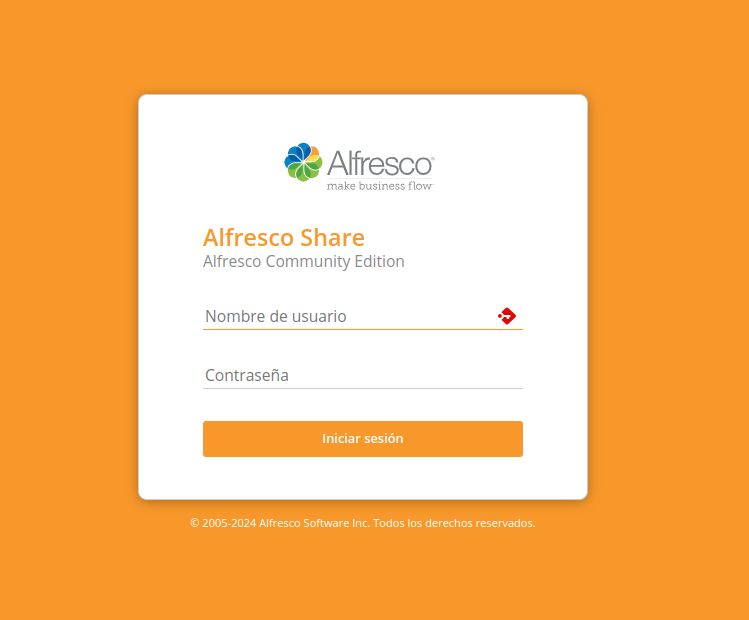
\includegraphics[width=\textwidth]{images/login}
		\label{fig:etiqueta_imagen}
	\end{figure}
	\item Haz clic en \textbf{Iniciar sesión} para acceder al panel principal de Alfresco Share.
\end{enumerate}

\subsection{Navegación básica en Alfresco Share}
Una vez que hayas iniciado sesión, te encontrarás en la interfaz principal de \textbf{Alfresco Share}. Aquí hay algunos elementos clave que te ayudarán a navegar:

\begin{itemize}
	\item \textbf{Barra de navegación:} Ubicada en la parte superior de la interfaz, permite acceder rápidamente a las diferentes áreas de Alfresco, como \textbf{Mis Archivos}, \textbf{Sitios}, \textbf{Repositorio}, y \textbf{Tareas}.
	\item \textbf{Panel de navegación lateral:} Situado a la izquierda, permite explorar la estructura de carpetas y sitios dentro de Alfresco, accediendo a documentos específicos y otras funcionalidades.
	\item \textbf{Barra de búsqueda:} Situada en la parte superior, permite buscar documentos, carpetas y sitios específicos dentro de Alfresco.
	\item \textbf{Área de contenido principal:} Aquí se muestra el contenido del área seleccionada en el panel de navegación, como archivos y carpetas en un sitio específico.
	\item \textbf{Menú de usuario:} En la esquina superior derecha, puedes acceder a tu perfil, configuraciones personales y la opción para cerrar sesión.
\end{itemize}

Familiarízate con estos elementos para moverte fácilmente por Alfresco y acceder a los documentos que necesitas firmar.

\subsection{Acceso a las funcionalidades de firma digital}
Para utilizar las funcionalidades de firma digital del plugin \textbf{Alfresco PDF Sign}, sigue estos pasos:

\begin{enumerate}
	\item Navega hasta el documento PDF que deseas firmar. Puedes hacerlo a través del \textbf{Repositorio} o accediendo al sitio correspondiente donde se almacena el documento.
	\item Haz clic derecho sobre el documento PDF para abrir el menú contextual.
	\item Selecciona la opción \textbf{Firmar documento PDF} (o la opción correspondiente configurada para el plugin) en el menú desplegable.
	\begin{figure}[h]
		\centering
		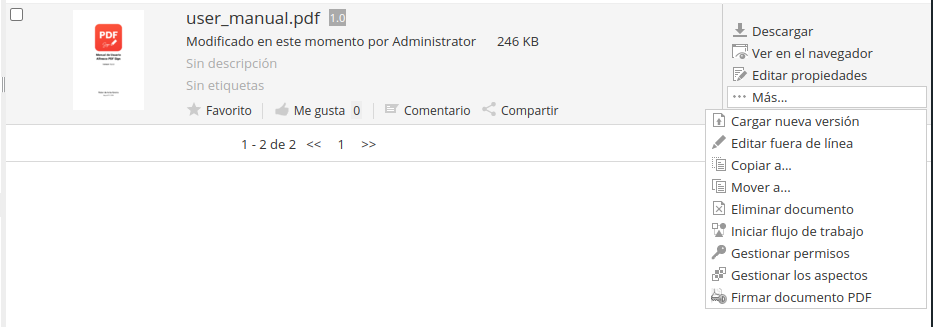
\includegraphics[width=0.85\textwidth]{images/sign-pdf}
		\label{fig:etiqueta_imagen}
	\end{figure}
	\item Se abrirá una interfaz que te permitirá seleccionar las opciones de firma, como el certificado digital, la página donde se aplicará la firma, y si la firma será visible o invisible.
	\begin{figure}[h]
		\centering
		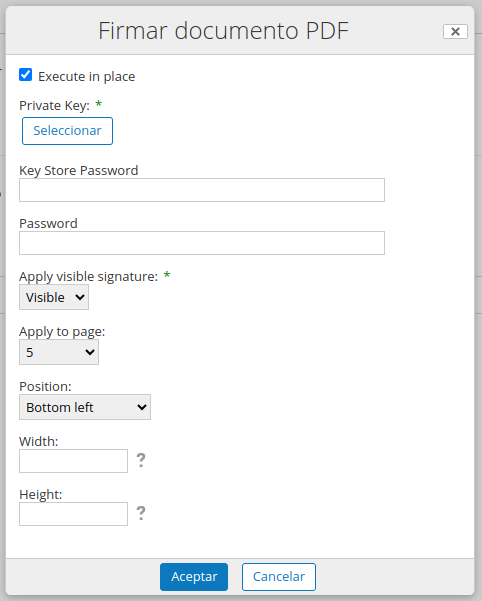
\includegraphics[width=0.5\textwidth]{images/sign-pdf2}
		\label{fig:etiqueta_imagen}
	\end{figure}
	\item \textbf{En la interfaz de firma que se abre, deberás configurar las siguientes opciones:}
	\begin{itemize}
		\item \textbf{Private Key:} Especifica la ruta donde se encuentra el archivo de la clave privada seleccionando \textit{Seleccionar} en el campo \textit{Private Key}.
		\begin{figure}[h]
			\centering
			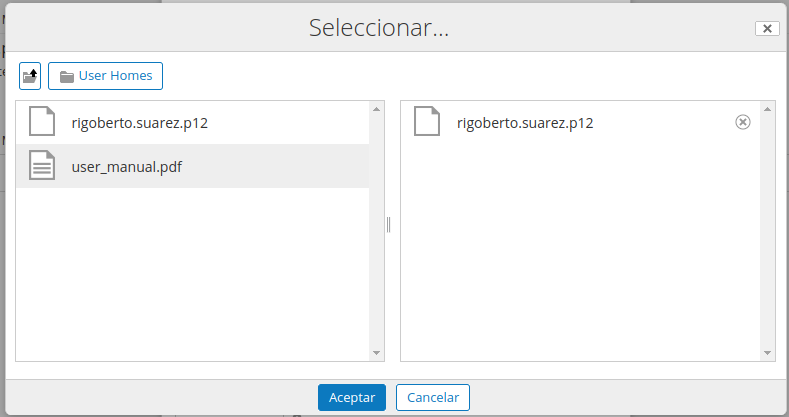
\includegraphics[width=0.85\textwidth]{images/private-key}
			\label{fig:etiqueta_imagen}
		\end{figure}
		\item \textbf{Key Store Password y Password:} Ingresa la contraseña específica para la firma en los campos correspondientes.
		
		\item \textbf{Ruta de destino para el documento firmado:}
		\begin{enumerate}
			\item Por defecto, la opción \textit{\textbf{Execute in place}} está marcada, lo que guardará el documento firmado en su ubicación actual.
			\item Si prefieres guardar el documento firmado en una ubicación diferente, desmarca \textit{\textbf{Execute in place}} y:
			\begin{itemize}
				\item \textbf{Destination name:} Especifica un nombre para el archivo firmado.
				\item \textbf{Destination folder:} Selecciona la carpeta donde deseas que se guarde el archivo firmado.
			\end{itemize}
		\end{enumerate}
		
		\item \textbf{Visibilidad de la firma:}
		\begin{itemize}
			\item Por defecto, la firma es visible. Si deseas que la firma sea oculta, selecciona \textit{Hidden} en el campo correspondiente.
		\end{itemize}
		
		\item \textbf{Página de la firma:}
		\begin{itemize}
			\item Por defecto, la firma se aplica en la última página del documento. Si prefieres firmar en una página específica, selecciona la página deseada en el menú desplegable.
			\item También tienes la opción de firmar en todas las páginas del documento escogiendo la opción \textit{All Pages}.
		\end{itemize}
		
		\item \textbf{Posición de la firma:}
		\begin{itemize}
			\item Selecciona la posición de la firma visible utilizando el menú desplegable \textit{Position}. Las opciones preestablecidas incluyen \textit{bottom left} (por defecto), \textit{top left}, entre otras.
			\item Si prefieres especificar manualmente la posición, puedes definir las coordenadas X y Y en los campos correspondientes.
			\item Opcionalmente, puedes ajustar el \textit{Width} (ancho) y \textit{Height} (altura) de la firma visible, aunque estos valores ya tienen un valor por defecto que se puede utilizar.
		\end{itemize}
	\end{itemize}
	
	\item \textbf{Completa los campos requeridos y haz clic en \textit{Firmar}} para aplicar la firma digital al documento.
	\item \textbf{Una vez que el documento haya sido firmado, este será marcado con un icono} que indica que ha sido firmado digitalmente. Este icono se puede ver junto al nombre del archivo en la interfaz de Alfresco, facilitando la identificación de documentos firmados.
	\begin{figure}[h]
		\centering
		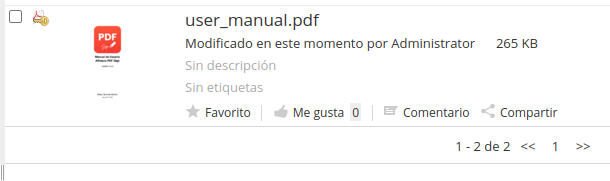
\includegraphics[width=0.85\textwidth]{images/signed-doc}
		\label{fig:etiqueta_imagen}
	\end{figure}
	\item \textbf{Si descargas y abres el documento PDF firmado, podrás ver que se ha añadido la firma solicitada} en la ubicación y con las características que seleccionaste durante el proceso de firma.
\end{enumerate}

\section{Firmas automáticas usando reglas de carpetas}
El plugin \textbf{Alfresco PDF Sign} permite automatizar el proceso de firma digital mediante la configuración de reglas en carpetas específicas. Esto es especialmente útil si deseas que todos los documentos que se agreguen a una carpeta se firmen automáticamente sin intervención manual. A continuación, te explico cómo configurar firmas automáticas usando reglas de carpetas en Alfresco.

\begin{enumerate}
	\item \textbf{Acceder a la carpeta para configurar la regla}
	\begin{itemize}
		\begin{figure}[h]
			\centering
			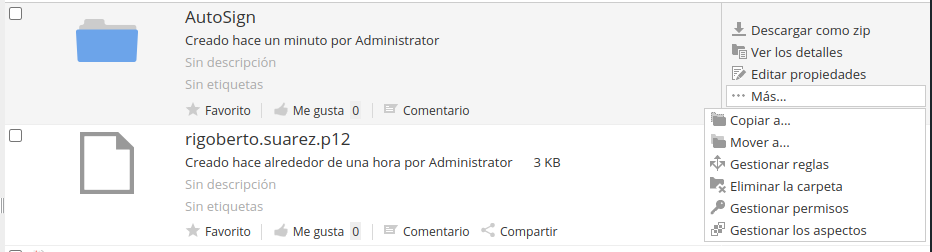
\includegraphics[width=0.82\textwidth]{images/rules}
			\label{fig:etiqueta_imagen}
		\end{figure}
		\item \textbf{Navega hasta donde se encuentra la carpeta deseada:} Accede hasta donde se encuentra la carpeta en la que deseas configurar la regla de firma automática. Puedes hacerlo a través del \textbf{Repositorio} o dentro de un sitio específico en Alfresco Share. No entres a la carpeta. 
		\item \textbf{Abrir el menú de reglas:} Haz clic derecho sobre la carpeta y selecciona \textit{Gestionar reglas} en el menú contextual. Esto te llevará a la página donde puedes crear y gestionar reglas para esa carpeta.
	\end{itemize}
	
	\item \textbf{Crear una nueva regla}
	\begin{itemize}
		\item \textbf{Añadir una nueva regla:} En la página de administración de reglas, haz clic en \textit{Crear regla} para comenzar a definir una nueva regla.
		\item \textbf{Añadir un nombre y una descripción a la regla:}  El nombre para la regla es obligatorio y la descripción si es opcional.
		\item \textbf{Definir cuando se va a ejecutar la regla:} Para una firma automática, selecciona \textit{Se crean o entran elementos en esta carpeta}
		\item \textbf{Definir criterio para la regla:} Seleccionar \textit{Todos los elementos} o especificar un criterio diferente.
		\item \textbf{Definir la acción a realizar:} Escoger la opción \textit{Sign PDF}.
		\item \textbf{Configurar las opciones de firma:} Configura los detalles de la firma de la misma manera que lo harías al firmar manualmente un documento. Esto incluye:
		\begin{itemize}
			\item \textbf{Private Key:} En lugar de especificar una ruta de archivo, debes proporcionar el \textit{nodeRef} del archivo que contiene la clave privada. \\ 
			{\small \textit{El nodeRef es un identificador único del archivo en Alfresco y tiene el formato workspace://SpacesStore/<UUID>. Puedes obtener el nodeRef desde la URL en la que se encuentra almacenada la clave privada.}}
			\item \textbf{Key Store Password y Password:} Ingresa la contraseña específica para la firma en los campos correspondientes.
			\item \textbf{Ruta de destino para el documento firmado:} Debe marcar la opción \textit{\textbf{Execute in place}}, lo que guardará el documento firmado en su ubicación actual. \\
			{\small \textit{Si prefiere guardar el documento luego de firmado en una ubicación diferente, desmarca \textit{\textbf{Execute in place}} y especifica un nombre para el archivo firmado en el campo \textbf{Destination name} y selecciona la carpeta donde deseas que se guarde el archivo firmado \textbf{Destination folder}.}}
			\item \textbf{Visibilidad de la firma:} Configura si la firma será visible o no.
			\item \textbf{Página de la firma:} Elige la página donde se aplicará la firma, por ejemplo: última página (\textbf{\textit{last}}), todas las páginas (\textbf{\textit{all}}), o una página específica (\textbf{\textit{1}}).
			\item \textbf{Posición de la firma:} Selecciona la posición de la firma visible utilizando el menú desplegable \textit{Position}. Las opciones preestablecidas incluyen \textit{bottom left} (por defecto), \textit{top left}, entre otras. \\
			{\small \textit{Si prefieres especificar manualmente la posición, puedes definir las coordenadas X y Y en los campos correspondientes.
			Opcionalmente, puedes ajustar el \textit{\textbf{Width}} (ancho) y \textit{\textbf{Height}} (altura) de la firma visible, aunque estos valores ya tienen un valor por defecto que se puede utilizar.}}
		\end{itemize}
		\begin{figure}[h]
			\centering
			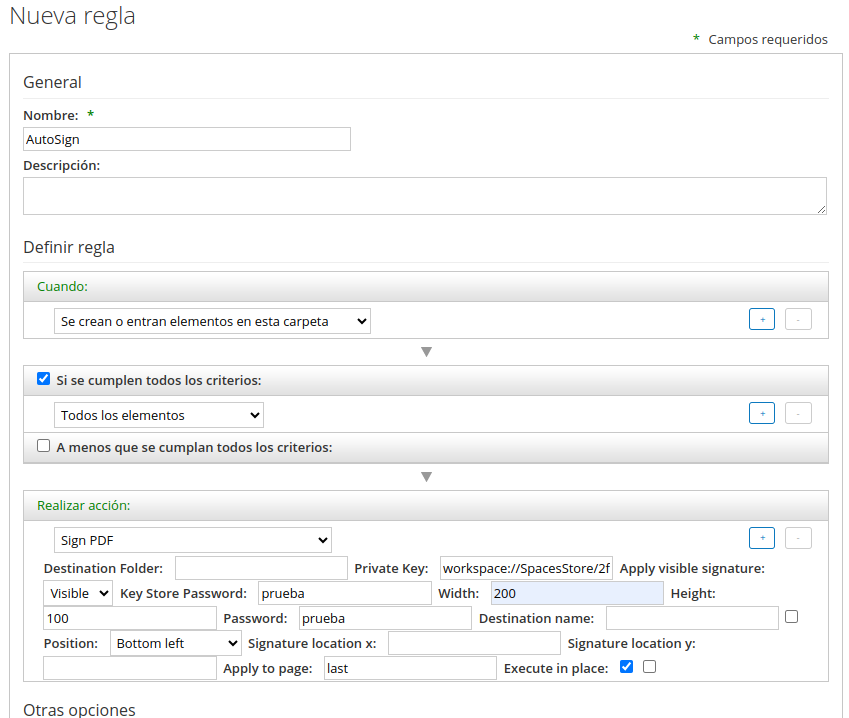
\includegraphics[width=0.8\textwidth]{images/rules2}
			\label{fig:etiqueta_imagen}
		\end{figure}
	\end{itemize}
	\item \textbf{Finalizar y guardar la regla}
	\begin{itemize}
		\item \textbf{Guardar la regla:} Una vez configuradas todas las opciones, haz clic en \textit{Guardar} para finalizar la creación de la regla. La regla aparecerá en la lista de reglas activas para esa carpeta.
		\item \textbf{Activar la regla:} Asegúrate de que la regla esté activada. Ahora, cada vez que se agregue un documento PDF a la carpeta, la regla aplicará automáticamente la firma digital según las configuraciones que has definido.
	\end{itemize}
	
	\item \textbf{Verificar la firma automática}
	\begin{itemize}
		\item \textbf{Agregar un documento PDF a la carpeta:} Suba o mueve un documento PDF a la carpeta con la regla configurada.
		\item \textbf{Verificar la firma:} Verifica que el documento ha sido firmado automáticamente revisando el icono de firma junto al archivo y abriendo el documento para comprobar la firma.
	\end{itemize}
\end{enumerate}

\section{Recursos adicionales}

Para aprovechar al máximo el plugin \textbf{Alfresco PDF Sign}, es esencial acceder a recursos adicionales que ofrecen soporte técnico, así como documentación y herramientas útiles. A continuación, se incluyen enlaces clave y opciones de soporte para ayudarte a resolver dudas, solucionar problemas, y optimizar el uso del plugin y la plataforma Alfresco.

\subsection{Documentación relacionada}

\begin{itemize}
	\item \textbf{Guía de usuario de Alfresco}\\
	Documentación oficial de Alfresco, incluyendo guías para usuarios, administradores y desarrolladores.\\
	\url{https://docs.alfresco.com/}
	
	\item \textbf{Documentación del plugin Alfresco PDF Sign}\\
	Información detallada sobre la instalación, configuración y uso del plugin en su repositorio de GitHub.\\
	\url{https://github.com/abraira85/alfresco-pdf-sign/tree/master/docs}
\end{itemize}

\subsection{Enlaces útiles}

\begin{itemize}
	\item \textbf{Repositorio GitHub del plugin Alfresco PDF Sign}\\
	Acceso al código fuente, releases y más información sobre el plugin.\\
	\url{https://github.com/abraira85/alfresco-pdf-sign}
	
	\item \textbf{Comunidad Alfresco}\\
	Foro y comunidad de usuarios y desarrolladores de Alfresco para compartir conocimientos y resolver dudas.\\
	\url{https://hub.alfresco.com/}
\end{itemize}

\section{Contacto}

Si tienes alguna pregunta, necesitas asistencia técnica, o deseas compartir tus comentarios sobre el plugin \textbf{Alfresco PDF Sign}, no dudes en ponerte en contacto con nosotros. Estamos aquí para ayudarte a sacar el máximo provecho de esta herramienta.

\begin{itemize}
	\item \textbf{GitHub}: Para reportar problemas, solicitar nuevas funcionalidades o contribuir al desarrollo del plugin, visita nuestro repositorio en GitHub: \url{https://github.com/abraira85/alfresco-pdf-sign}
\end{itemize}

Tu feedback y participación son esenciales para mejorar continuamente el plugin y asegurarnos de que cumpla con tus necesidades.


\end{document}
